\chapter{Чем легионер отличается от крестьянина?}

Многим кажется что "война никогда не меняется", она всегда однозначно Адъ и Израилъ. А несчастные люди, которых занесло туда — по умолчанию жертвы. Кто бы они не были, от случайных прохожих и до высшего командного состава. Но это не совсем так. Наше представление в войне сформировано чудовищными мясорубками последних столетий, где бенефициары войн сидят по уютным кабинетам и считают шекели или молятся на какой-то очередной "изм", во имя которого они готовы пустить на дымящийся фарш кого угодно А в окопах люди в лучшем случае "выполняют свой долг и защищают Родину", а в худшем вообще не понимают что происходит. Это беда массовых призывных армий, когда в мясорубку затягивает, де-факто, случайных людей. Мобилизовали тебя, ты куда-то пошел, чет делаешь, потом бац и всё, гейм овер. Ну или ты научишься прыгать от смерти достаточно успешно и доживешь до конца, где тебе дадут шоколадную медаль и отправят домой, дальше сапать грядки.


Совсем другое дело когда бенефициар войны это ты. А так как паблик у нас исторический, то проиллюстрируем на примере, сравнив марианского легионера и призывного батрака времен Раннего Средневековья. Поехали. 	

\begin{figure}[h!tb]
	\centering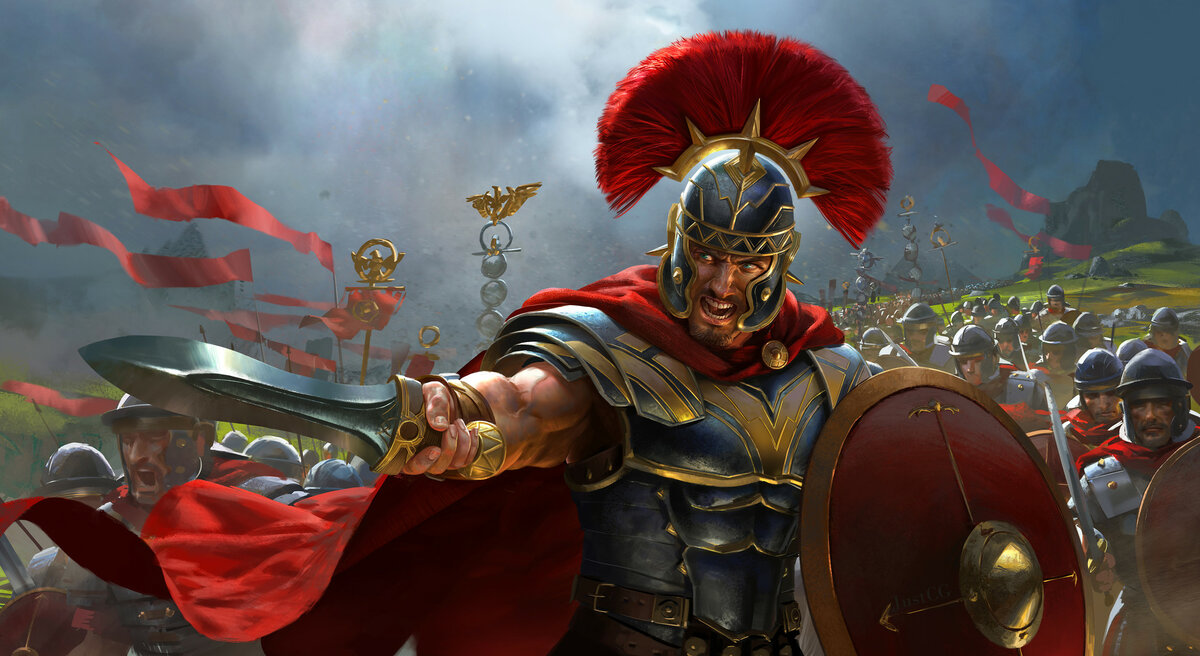
\includegraphics[scale=0.3]{Legioner/1594657934178989633.png}
	\label{fig:leg1} % Unique label used for referencing the figure in-text
	%\addcontentsline{toc}{figure}{Figure \ref{fig:placeholder}} % Uncomment to add the figure to the table of contents
	%	\caption{Митридат и его периферийный гегемон наглядно. Неудачно, но тем не менее. Рядом отожравшаяся на трупе Селевкидов Парфия. }
\end{figure}



Вот ты легионер, записался от безделья и безденежья в армию и сумел пережить "курс молодого бойца". Где из тебя вышибли всё мешающее служить твоей любимой Республике, вместе с той половиной мозга, которая римскому военному не требуется. Теперь перед тобой открываются поистине сказочные перспективы, о которых ты и мечтать не мог. Во-первых, все твои бытовые и денежные неурядицы закончились навсегда. Легион о тебе позаботится, оденет, накормит и обеспечит приказами вышестоящего командования, выполнять которые теперь - твой новый смысл жизни лет на двадцать, пока Республика не скажет "малаца" и не отправит тебя на пенсию. Жалование тебе платит сам император, лично, и поэтому спиздить твои деньги не просто нельзя, а за это головы рубят. На своё жалование ты всегда можешь купить себе пожрать, и как минимум лепешек с мясом наделать, плюс фруктов каких накупить. Снабжается армия централизовано и, по меркам времени, достаточно хорошо, ведь Империи нужно чтоб ты хорошо кушал, иначе ослабнешь, заболеешь и сдохнешь от кровавого поноса. 
Плюс на границах легионер часто вообще единственный покупатель, способный платит монетой (император\_платит, напоминаю), и это открывает свои перспективы. Всё снаряжение ты получаешь централизовано из арсенала, ведь ты должен быть хорошо вооружен, иначе тебя убьют нахуй, а это никому не нужно. 
Правда, чинить снарягу и менять по мере износа придется за свой счет, точить оружие, менять износившиеся ремешки и подновлять краску на щите (унифицированные алые-оранжевые расцветки это более поздний мем, на самом деле каждый легион красил себе щиты в меру своей фантазии, были даже белые). Но денег тебе на это хватает, да и все нужные мастера есть в самом легионном лагере. Ну а если ты гдет проебал свой комплект силовой боевой брони модель два, то его стоимость будет вычтена из твоего жалования, а в арсенале выдадут новый комплект и можешь быть свободен, тут нет никакой проблемы.


Но это всё быт, главное тут другое. Легион - твоя семья, он не только обеспечивает тебя всем необходимым, но и решает всякие экзистенциальные вопросы про смысл жизни и прочие сложные материи. Сначала они решаются тем, что твой центурион хуярит тебя стимулом (так называлась палка, которой младшие командиры стимулировали солдат) по голове, но потом ты и сам перестаешь их себе задавать. Минимальная организационная единица легиона - контуберния, 8-10 человек, живущих в одной палатке, ведущих общий быт, скидывающихся на хавчик и всякие предметы общего пользования. Во главе контубернии стоял декан (decanus), десятник на наши деньги, наиболее толковый и уважаемый ветеран, и это первая ступенька, на которую можно забраться в иерархии. Ну а дальше можно было к концу службы дослужится и до Первого Центуриона, что автоматически переводит тебя в совершенно другой социальный кластер (центурионы Цезаря после пары лет войн виллы скупали на время увольнительных просто чтобы награбленное непосильным трудом без дела не болталось). Легион дает тебе свою, так сказать, линейку прокачки и заботится о тебе на всех уровнях. Твой центурион (как только выбьет стимулом у тебя из башки всякую чушь и ты станешь минимально толковым военным) будет говорить тебе "Люций хороший" и знать какие у тебя любимые стикеры. Ты не расходник, ты легионер Ранней Империи, идеальное оружие в руках самого могучего государства Ойкумены.


"Ну а если война?", спросит читатель. А если война, то значит на твоей улице праздник. Можешь смело грохнуть чарку-другую хорошего вина, восславив мудрого императора, который начал войну с кем-нибудь, или недальновидного противника, который сам спровоцировал Империю на своё уничтожение. Если твоя жизнь в относительно мирное время была неплоха, то с началом боевых действий наступают по настоящему хорошие деньки. Война это развлечение (служба это ведь всегда скучно, во все времена), война это обогащение (даже в небольшой кампании можно стать очень богатым человеком, ведь можно грабить), война это карьерный рост (и за счет потерь и за счет взрывного роста армии), ну и просто война — это то, к чему тебя готовили всё это время. Если легион это твоя семья, то война — это твой дом, где не твоя жизнь в опасности, а ты и есть опасность. "Кому война а кому мать родна", так сказать. Кто-то там как теленок на бойне, а кто-то её недоношенный ребенок, надо понимать разницу.


\begin{figure}[h!tb]
	\centering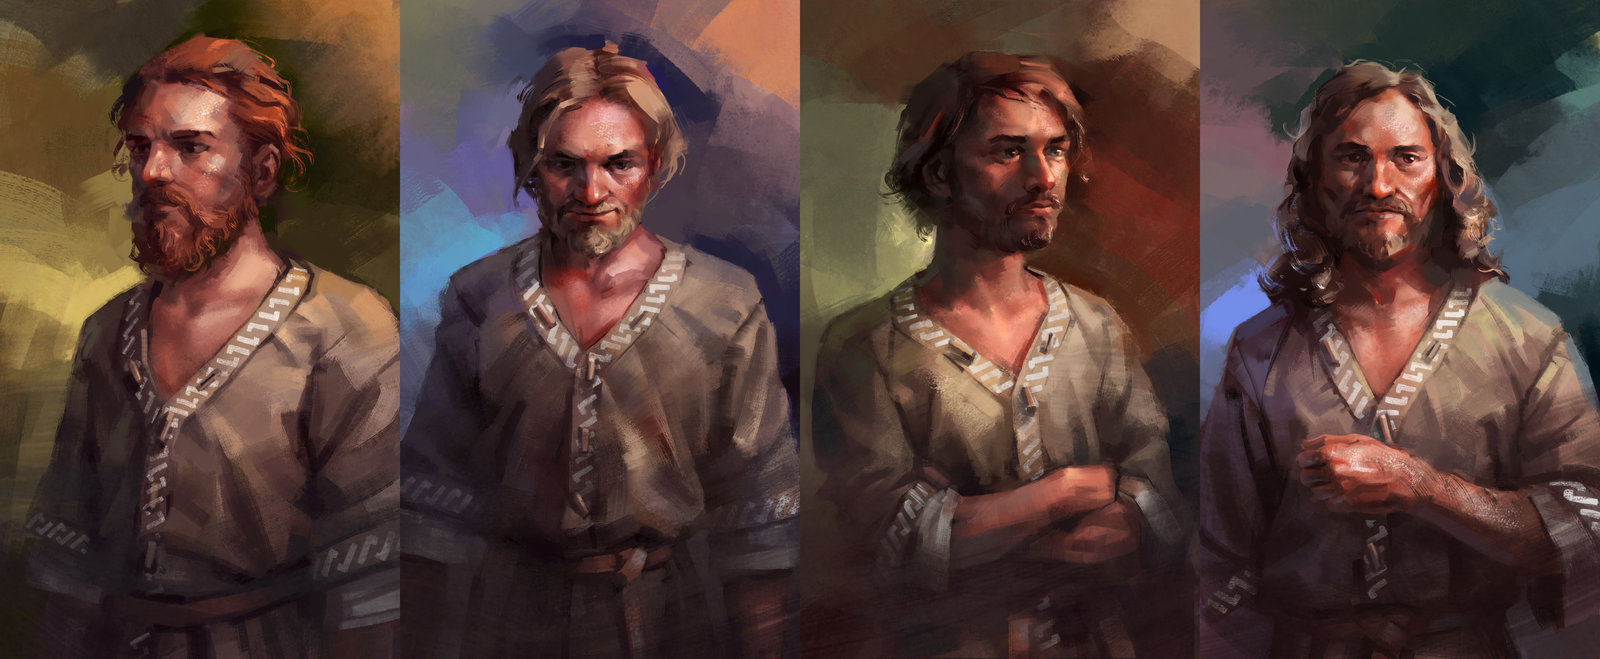
\includegraphics[scale=0.3]{Legioner/1594658107116371201.png}
	\label{fig:leg2} % Unique label used for referencing the figure in-text
	%\addcontentsline{toc}{figure}{Figure \ref{fig:placeholder}} % Uncomment to add the figure to the table of contents
	%	\caption{Митридат и его периферийный гегемон наглядно. Неудачно, но тем не менее. Рядом отожравшаяся на трупе Селевкидов Парфия. }
\end{figure}



И вот теперь давайте отвлечемся от нашего легионера и посмотрим в завтрашний день, где копает грядки с брюквой какой-нибудь Жак. В деревню этого самого Жака приходят вербовщики от сэра Ланселота (вставьте сюда подходящую титулатуру, я не придумал), и набирают себе этих жаков сколько получается, с расчетом на то, чтобы в деревне было кому продолжить копать брюкву, но не более. После чего ничего не понимающему Жаку дают дрын, учат им махать пару часов и ставят в строй. Где он, собственно, стоит и охуевающе пучит глаза на налетающую волну кавалерии, пытается не обосраться и не потерять свой дрын. Затем кавалерия сметает этих жаков и размазывает их по полю тонким слоем, начинается какой-то кровавый хаос и наш герой тычет куда-то своей палкой, пытаясь выжить и молясь Деве Марии о возвращении к своей брюкве. Допустим Жак выжил, и его армия даже победила, ура-ура. Ну, теперь Жаку самое время идти куда-то (и постараться не умереть от дизентерии по дороге), куда скажут, на следующее поле боя или осаду, и уже там куда-то бежать, чего-то орать и размахивать своим дрыном пока вокруг происходит кромешный адъ. Если всё пойдет хорошо, то война закончится через пару месяцев, а Жака, отпустят домой, ведь осень же, пора брюкву собирать. Он, собственно, и пойдет её собирать, а потом перезимует и снова весна, а значит сначала посевная, а потом сэры ланселоты начинают меряться хуями и вербовщики опять отлавливают жаков по деревням, так как кто-то ведь должен умереть за "наше великое дело" на непонятной и ненужной простому Жаку войне.


Вот такая хуйня, малята. Можно тут встать и заявить что "и легионер может в какой-нибудь осаде черепом кусок черепицы поймать и сдохнуть". Но легионер-то готов к этому. А мобилизованный крестьянин — нет. Легионера государство взяло "на попечение", научило и обеспечило, теперь "его дом — война, его работа — убивать". И оно их использует по прямому назначению. А батраков просто согнали на бойню, разменяли на таких же на другой стороне и збс, смыть-повторить. "Герцог с бароном сцепились по пьяни и завалили всё поле боя трупами крестьян, каждый год одно и то же", хехе. И умирая не дожив до пенсии Люций просто взгрустнет от того что не удалось прикупить маленький домик в Кампании и сидеть, попивать винишко на крыльце, смотря как малолетние латины ебашат друг друга деревянными мечами. А Жак перед смертью подумает "еб вашу мать, что тут вообще происходит, можно не надо погибать хуй пойми за что". Такие вот дела, два мира, два шапито. При этом учитывайте что я нарисовал тут портреты ТИПИЧНЫХ военных той и другой эпохи. Большая часть античных армий так или иначе состояла из Люциев, военных профессионалов, понимающих на что они подписались. А большая часть средневековых армий это одноразовые Жаки, которые каждый год новые и "бабы ещё нарожают". И именно поэтому люблю я античку и её военную историю, а всё это средневековое фехтование крестьянами мне кажется каким-то мрачным, безысходным говном, от которого лучше держаться подальше чисто из соображений "моральной гигиены".

%\begin{figure}[h!tb]
%	\centering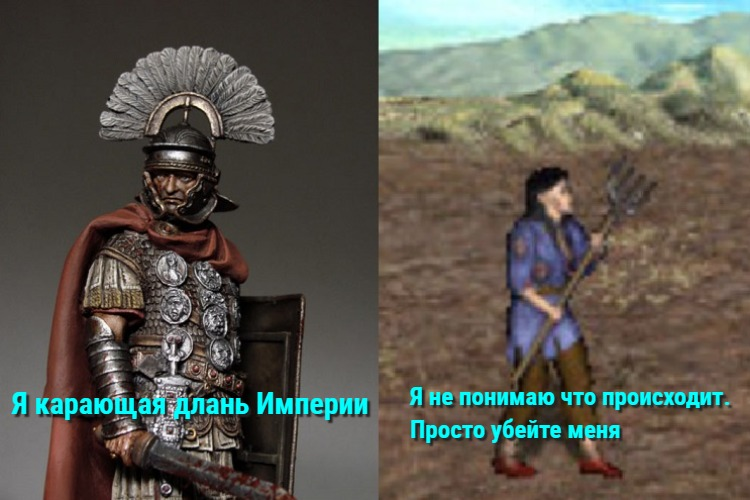
\includegraphics[scale=0.5]{Legioner/1594658137151640534.png}
%	\label{fig:leg3} % Unique label used for referencing the figure in-text
%	%\addcontentsline{toc}{figure}{Figure \ref{fig:placeholder}} % Uncomment to add the figure to the table of contents
%	%	\caption{Митридат и его периферийный гегемон наглядно. Неудачно, но тем не менее. Рядом отожравшаяся на трупе Селевкидов Парфия. }
%\end{figure}
